\section{Experimentacion}
\subsection{Busqueda exhautiva}
Para la realizacion de los experimientos implementamos un algoritmo de busqueda exhautiva para buscar el mejor modelo en cada caso. 

El algoritmo es el siguiente:

\begin{lstlisting}[caption=grid\_search]
def grid_search(param_grid):
	grid = ParameterGrid(param_grid)
	best_error = None
	best_params = None
	print "Ejercicio "+str(param_grid["1"])
	print len(grid), "modelos distintos"
	i = 0
	print "i 	error(training, validacion)"
	start = timer()
	for params in grid:
	    e = train(params['1'], params['2'], params['3'],params['4'],params['5'],params['6'],params['7'],
	    	params['8'],params['9'],params['10'],params['11'], True )
	    print i, "	", e
	    i += 1
	    if i%50 == 0:
	    	end = timer()
	    	print int((end-start)/60), " min"
	    if best_error == None or e < best_error:
	    	best_error = e
	    	best_params = [params['1'], params['2'], params['3'],params['4'],params['5'],params['6'],params['7'],params['8'],
	    	params['9'],params['10'],params['11']]
	print "MEJOR ERROR Y MODELO EJERCICIO "+str(param_grid["1"])
	print "training, validacion:", best_error
	print "parametros:", best_params
	end = timer()
	print int((end-start)/60), " min"
\end{lstlisting}

Y la forma de instanciarlo es la siguiente:

\begin{lstlisting}[caption=Instanciacion]
param_grid = {'1': [1],"2":['./datasets/tp1_ej1_training.csv'],"3": [None], "4":[0.1], "5": [200], 
			"6":[0.001,0.01,0.1,0.5, 0.005, 0.2, 0.3, 0.4], "7":[0.1,0.3,0.5, 0.7, 0.9], "8": [0.70], 
			"9": [0,1], "10":[0], "11":[[5],[10],[15],[20],[25],[15,15],[5,5],[10,10]]}
\end{lstlisting}

La idea es bastante simple, lo que hacemos es pasar por parametro una lista con todos los posibles para parametros y el algoritmo corre un ciclo, donde en cada ciclo prueba con un parametro distinto guardandoce el mejor modelo para finalmente imprimirlo por la consola.

De esta forma logramos quedarnos con la mejor arquitectura en cada ejercicio. PERO DE TODAS FORMAS, HICIMOS PRUEBAS MANUALES PARA VALIDAD QUE ESTO ERA CIERTO Y PARA ESTO HICIMOS EL SIGUIENTE ANALISIS.
\subsection{Ejercicio 1}

Observamos que agregar capas no garantiza la convergencia y, cuando lo hace, provoca que las salidas oscilen abruptamente y tarde mas epocas, por lo que optamos por utilizar dos capas ocultas como compromiso entre tiempo y calidad de solucion. 

En cuanto al numero de unidades por capa, ejecutamos el grid\_search 10 veces y en total encontramos que una buena solucion es:

\begin{enumerate}
\item epsilon: 0.1
\item tau: 200
\item etha: 0.01
\item momentum: 0.9
\item holdoutRate: 0.7
\item modo: Incremental
\item unidades por capa: 5 y 5
\end{enumerate}

Y para esta obtuvimos los siguientes graficos.


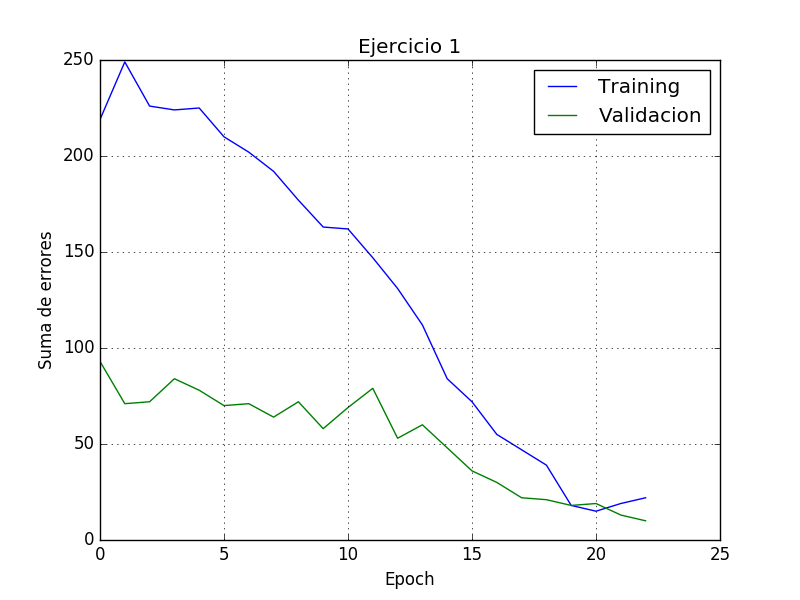
\includegraphics[scale=0.4]{img/ej100109155sum}
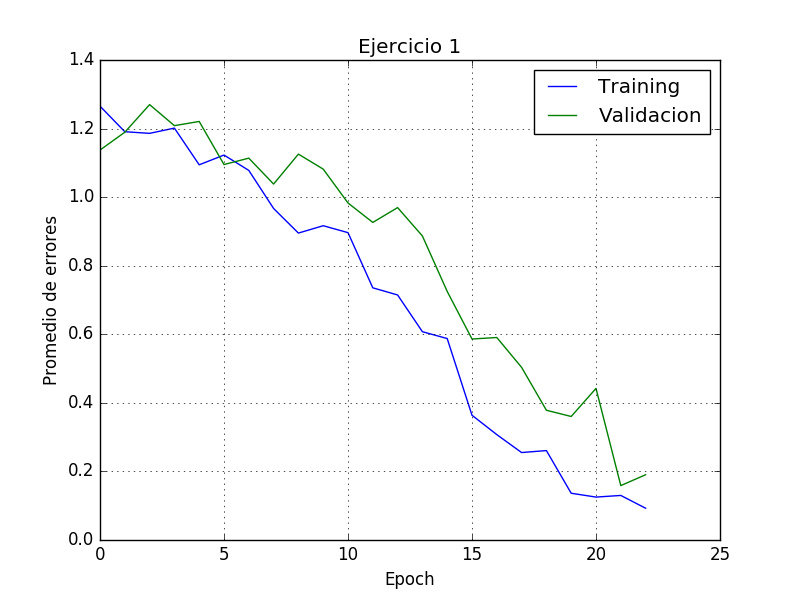
\includegraphics[scale=0.4]{img/ej100109155mean}

En estos graficos podemos ver BLA BLA BLA BLA.


Sin embargo, al mirar los graficos de error, nos dimos cuenta que la solucion de 5 neuronas no converge en general.
Como el campo de busqueda es pequeno, probamos multiples veces diferentes configuraciones de neuronas con numeros de 2 a 15 neuronas por capa para tener una evidencia estadistica de que sucede al variar este parametro. Con ello corroboramos que la solucion arrojada por el algoritmo de busqueda estaba cerca de un resultado optimo al ver las variaciones de diferentes medidas de error. 

Las medidas de error que tomamos fue el numero de unidades con error, el error total, el promedio de error, condicion de terminacion de aprendizaje, es decir, si termino por error menor a epsilon o por limite de epocas. En particular, por la naturaleza del problema, nos interesa ver la Precisión y el Recall, o dicho de otra manera, el indice de falso positivo y falso negativos. 

Como medida utilizaremos la Media armónica donde 

Media armonica=2*precision*recall/(precision+recall)

precision=true positive/(true positive+false positive)

recall= true positive/(true positive+false negative)


Para determinar el valor de la primer capa, elegimos aquellas configuraciones que nunca terminen debido al limite de epocas. Luego, en base a la cantidad de unidades con error y el error total cometido, las clasificamos en este orden. 
En particular, obtuvimos que las configuraciones de [8,7] y [9,5] arrojan buenos resultados.

Podemos ver a continuacion algunos graficos obtenimos variando los parametros con 8 y 7 capas.

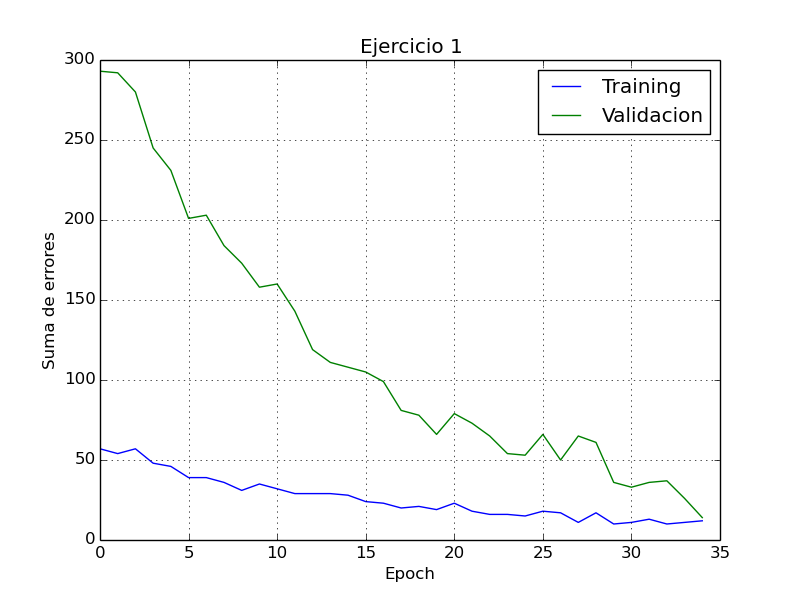
\includegraphics[scale=0.4]{img/ej100207187sum}
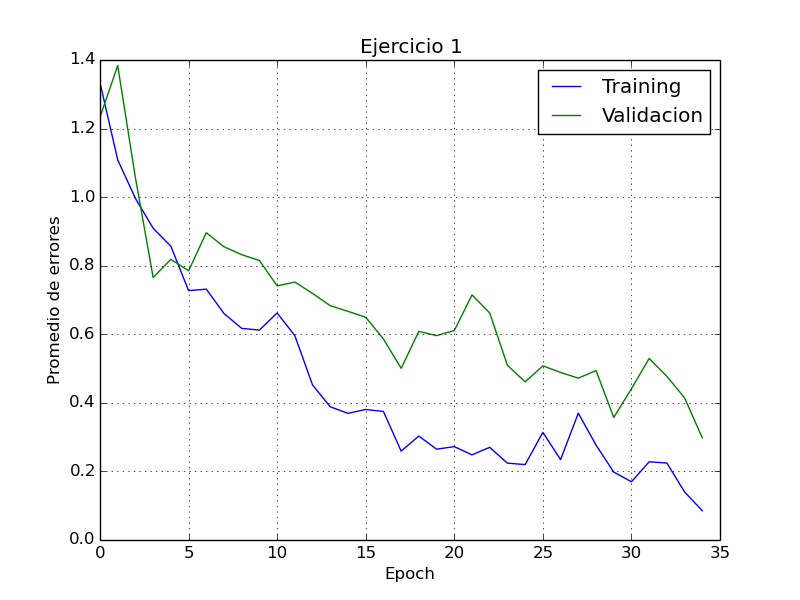
\includegraphics[scale=0.4]{img/ej100207187mean}

En particular este grafico fue el mejor de los graficos que obtuvimos variando los parametros para esta cantdiad de capas. Y los parametros son:
\begin{enumerate}
\item epsilon: 0.1
\item tau: 200
\item etha: 0.02
\item momentum: 0.7
\item holdoutRate: 0.7
\item modo: Incremental
\item unidades por capa: 8 y 7
\end{enumerate}

Se puede ver en estos graficos que...

Podemos ver a continuacion algunos graficos obtenimos variando los parametros con 9 y 5 capas.


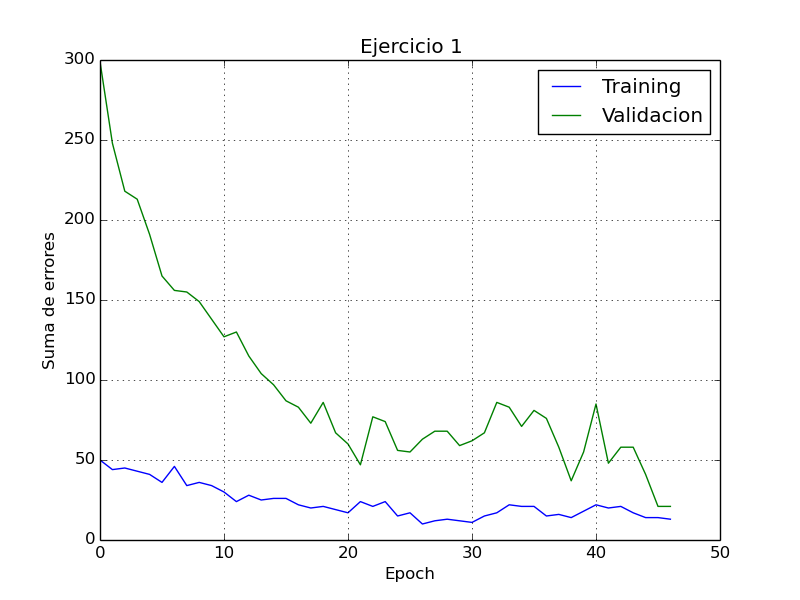
\includegraphics[scale=0.4]{img/ej100505195sum}
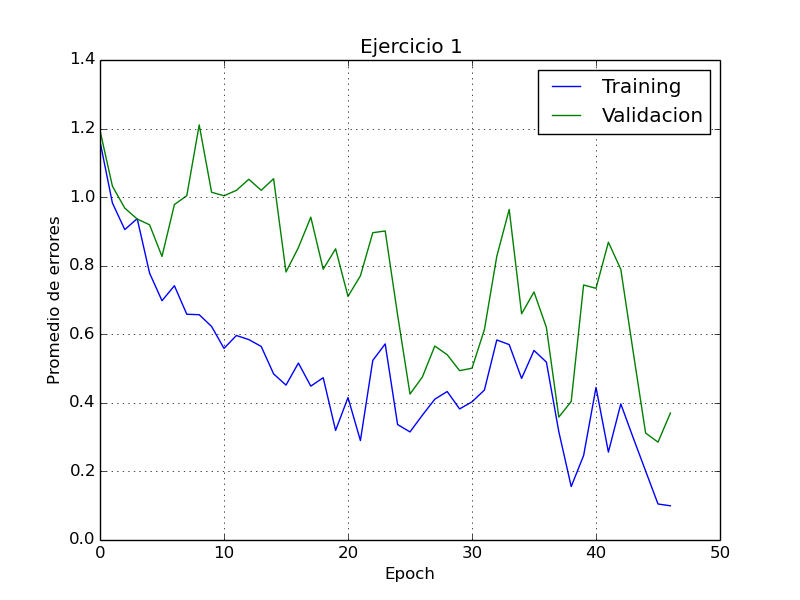
\includegraphics[scale=0.4]{img/ej100505195mean}


En particular este grafico fue el mejor de los graficos que obtuvimos variando los parametros para esta cantdiad de capas. Y los parametros son:
\begin{enumerate}
\item epsilon: 0.1
\item tau: 200
\item etha: 0.05
\item momentum: 0.5
\item holdoutRate: 0.7
\item modo: Incremental
\item unidades por capa: 9 y 5
\end{enumerate}

Se puede ver a continuacion que...

En conclusion, decidimos elegir como modelo el de 5 y 5 capas dado que es el que tiene menor cantidad de capas y por lo tanto menor procesamiento.

Por ultimo, graficamos un histograma para ver la cantidad de equivocaciones a la hora de predecir si un cancer es benigno o maligno.

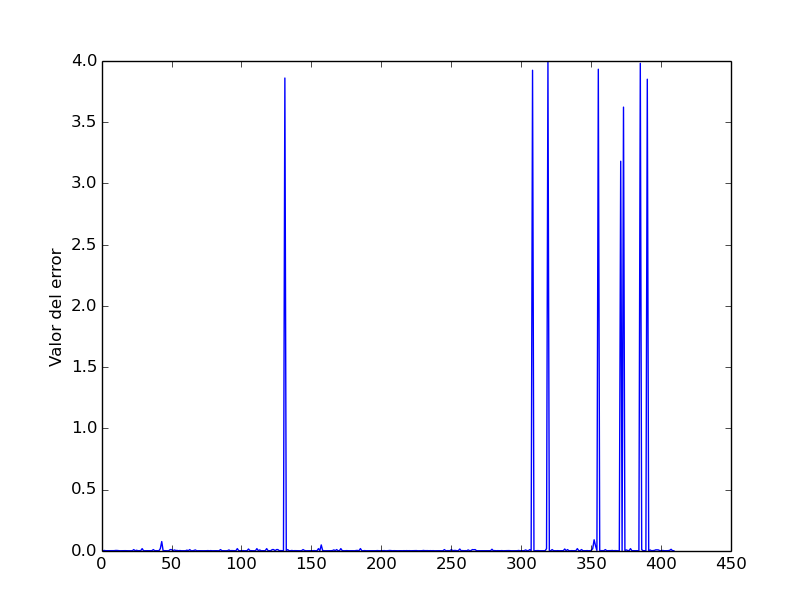
\includegraphics[scale=0.7]{img/histogramaej155}

Se puede ver en el grafico que la cantidad de equivocaciones es 8, siendo este un numero muy chico ya que la cantidad de muestras es de 500.


\subsection{Ejercicio 2}

Al igual que en el ejercicio 1, en este ejercicio se corrio el algoritmo de grid\_search 10 veces y en total encontramos que una buena solucion es:

\begin{enumerate}
\item epsilon: 0.1
\item tau: 200
\item etha: 0.005
\item momentum: 0.9
\item holdoutRate: 0.7
\item modo: Incremental
\item unidades por capa: 5
\end{enumerate}

Y para esta obtuvimos los siguientes graficos.

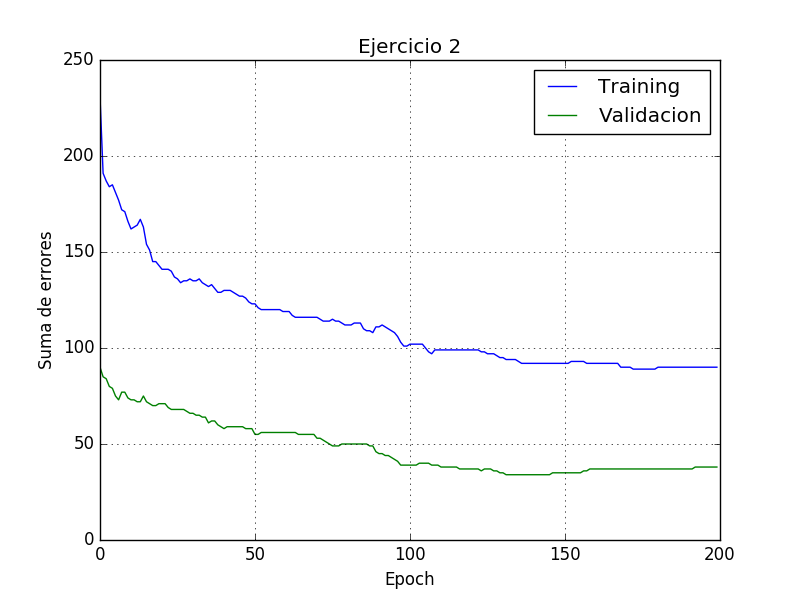
\includegraphics[scale=0.4]{img/ej200050915sum}
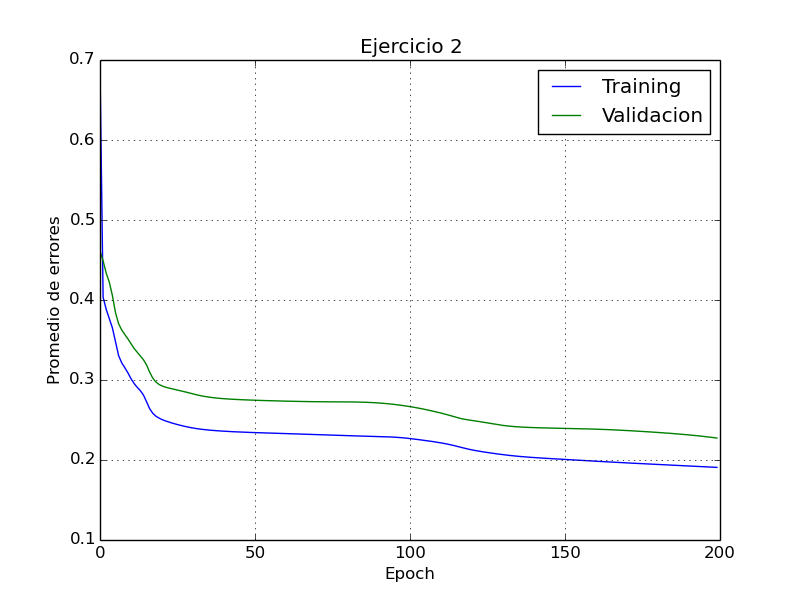
\includegraphics[scale=0.4]{img/ej200050915mean}

Se puede ver en estos graficos que...


\subsection{Conclusion}
